
\documentclass[tikz,border=8mm]{standalone}
\usepackage[T1]{fontenc}
\usepackage[utf8]{inputenc}
\usepackage{lmodern}
\usepackage{amsmath}
\usepackage{xcolor}
\usetikzlibrary{arrows.meta,calc,positioning}

\definecolor{Title}{HTML}{263442}
\definecolor{Accent}{HTML}{4F6F82}
\definecolor{Grid}{HTML}{74818C}
\definecolor{TextSoft}{HTML}{52606D}
\definecolor{Acol}{HTML}{D8E9FA}
\definecolor{Bcol}{HTML}{D9EED2}
\definecolor{Ccol}{HTML}{F7E7B3}
\definecolor{Dcol}{HTML}{E8D4F0}

\begin{document}
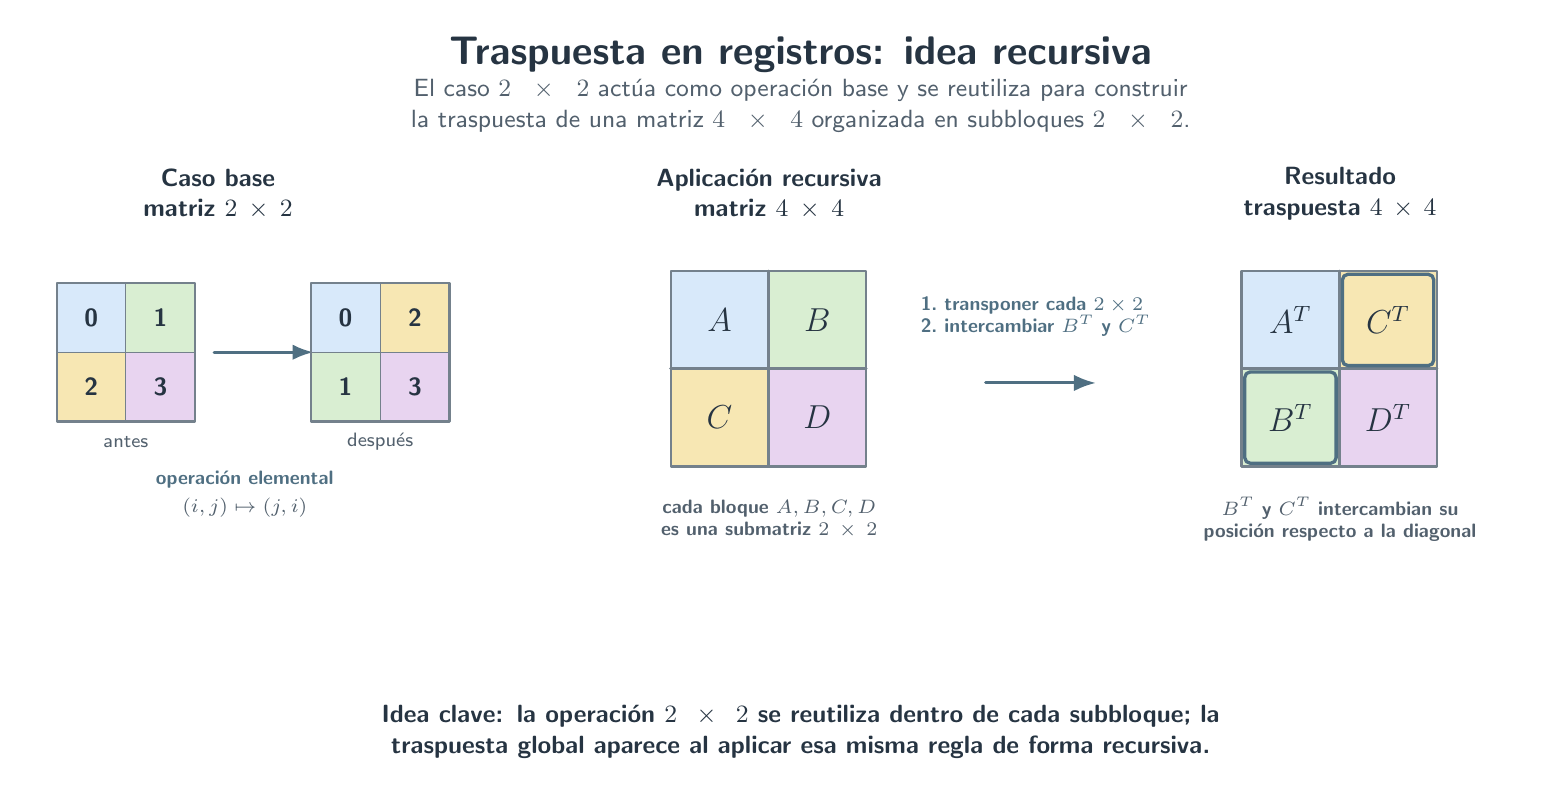
\begin{tikzpicture}[
  x=1cm,y=1cm,
  line cap=round,
  line join=round,
  >={Latex[length=2.3mm,width=1.7mm]}
]

% ================================================================
% Título
% ================================================================
\node[
  font=\sffamily\bfseries\Large,
  text=Title,
  align=center
] at (10.4,9.95)
{Traspuesta en registros: idea recursiva};

\node[
  font=\sffamily\small,
  text=TextSoft,
  align=center,
  text width=17.6cm
] at (10.4,9.30)
{El caso $2\times2$ actúa como operación base y se reutiliza para construir
la traspuesta de una matriz $4\times4$ organizada en subbloques $2\times2$.};

% ================================================================
% Encabezados
% ================================================================
\node[
  font=\sffamily\bfseries\small,
  text=Title,
  align=center,
  text width=4.6cm
] at (3.00,8.18)
{Caso base\\matriz $2\times2$};

\node[
  font=\sffamily\bfseries\small,
  text=Title,
  align=center,
  text width=4.8cm
] at (10.00,8.18)
{Aplicación recursiva\\matriz $4\times4$};

\node[
  font=\sffamily\bfseries\small,
  text=Title,
  align=center,
  text width=4.8cm
] at (17.25,8.18)
{Resultado\\traspuesta $4\times4$};

% ================================================================
% Caso base 2x2
% ================================================================
\def\s{0.88}
\def\xA{0.95}
\def\yA{7.05}

\fill[Acol] (\xA,\yA) rectangle ++(\s,-\s);
\fill[Bcol] (\xA+\s,\yA) rectangle ++(\s,-\s);
\fill[Ccol] (\xA,\yA-\s) rectangle ++(\s,-\s);
\fill[Dcol] (\xA+\s,\yA-\s) rectangle ++(\s,-\s);

\draw[Grid,line width=0.75pt] (\xA,\yA) rectangle ++(2*\s,-2*\s);
\draw[Grid,line width=0.42pt] (\xA+\s,\yA) -- ++(0,-2*\s);
\draw[Grid,line width=0.42pt] (\xA,\yA-\s) -- ++(2*\s,0);

\node[font=\sffamily\small\bfseries,text=Title] at (\xA+0.5*\s,\yA-0.5*\s) {0};
\node[font=\sffamily\small\bfseries,text=Title] at (\xA+1.5*\s,\yA-0.5*\s) {1};
\node[font=\sffamily\small\bfseries,text=Title] at (\xA+0.5*\s,\yA-1.5*\s) {2};
\node[font=\sffamily\small\bfseries,text=Title] at (\xA+1.5*\s,\yA-1.5*\s) {3};

\node[font=\sffamily\scriptsize,text=TextSoft]
  at (\xA+\s,\yA-2*\s-0.26) {antes};

\draw[-Latex,Accent,line width=1.0pt]
  (\xA+2*\s+0.24,\yA-\s) -- ++(1.26,0);

\def\xB{4.18}

\fill[Acol] (\xB,\yA) rectangle ++(\s,-\s);
\fill[Ccol] (\xB+\s,\yA) rectangle ++(\s,-\s);
\fill[Bcol] (\xB,\yA-\s) rectangle ++(\s,-\s);
\fill[Dcol] (\xB+\s,\yA-\s) rectangle ++(\s,-\s);

\draw[Grid,line width=0.75pt] (\xB,\yA) rectangle ++(2*\s,-2*\s);
\draw[Grid,line width=0.42pt] (\xB+\s,\yA) -- ++(0,-2*\s);
\draw[Grid,line width=0.42pt] (\xB,\yA-\s) -- ++(2*\s,0);

\node[font=\sffamily\small\bfseries,text=Title] at (\xB+0.5*\s,\yA-0.5*\s) {0};
\node[font=\sffamily\small\bfseries,text=Title] at (\xB+1.5*\s,\yA-0.5*\s) {2};
\node[font=\sffamily\small\bfseries,text=Title] at (\xB+0.5*\s,\yA-1.5*\s) {1};
\node[font=\sffamily\small\bfseries,text=Title] at (\xB+1.5*\s,\yA-1.5*\s) {3};

\node[font=\sffamily\scriptsize,text=TextSoft]
  at (\xB+\s,\yA-2*\s-0.26) {después};

\node[
  font=\sffamily\scriptsize\bfseries,
  text=Accent,
  align=center
] at (3.34,4.55)
{operación elemental};

\node[
  font=\sffamily\scriptsize,
  text=TextSoft,
  align=center
] at (3.34,4.20)
{$(i,j)\mapsto(j,i)$};

% ================================================================
% Reutilización recursiva
% ================================================================\node[
  font=\sffamily\scriptsize\bfseries,
  text=Accent,
  align=center,
  fill=white,
  inner sep=1.5pt
] at (6.55,5.95)
{reutilización recursiva};

% ================================================================
% Matriz 4x4 por subbloques 2x2
% ================================================================
\def\c{0.62}
\def\mx{8.75}
\def\my{7.20}

\fill[Acol] (\mx,\my) rectangle ++(2*\c,-2*\c);
\fill[Bcol] (\mx+2*\c,\my) rectangle ++(2*\c,-2*\c);
\fill[Ccol] (\mx,\my-2*\c) rectangle ++(2*\c,-2*\c);
\fill[Dcol] (\mx+2*\c,\my-2*\c) rectangle ++(2*\c,-2*\c);

\draw[Grid,line width=0.90pt] (\mx,\my) rectangle ++(4*\c,-4*\c);
\draw[Grid,line width=1.12pt]
  (\mx+2*\c,\my) -- ++(0,-4*\c);
\draw[Grid,line width=1.12pt]
  (\mx,\my-2*\c) -- ++(4*\c,0);

\node[font=\sffamily\bfseries\large,text=Title] at (\mx+\c,\my-\c) {$A$};
\node[font=\sffamily\bfseries\large,text=Title] at (\mx+3*\c,\my-\c) {$B$};
\node[font=\sffamily\bfseries\large,text=Title] at (\mx+\c,\my-3*\c) {$C$};
\node[font=\sffamily\bfseries\large,text=Title] at (\mx+3*\c,\my-3*\c) {$D$};

\node[
  font=\sffamily\scriptsize,
  text=TextSoft,
  align=center,
  text width=4.8cm
] at (10.00,4.05)
{cada bloque $A,B,C,D$ es una submatriz $2\times2$};

% ================================================================
% Paso global
% ================================================================
\draw[-Latex,Accent,line width=1.10pt]
  (12.75,5.78) -- (14.15,5.78);

\node[
  font=\sffamily\scriptsize\bfseries,
  text=Accent,
  align=left,
  text width=3.05cm,
  fill=white,
  inner sep=1.5pt
] at (13.45,6.62)
{1.\ transponer cada $2\times2$\\
 2.\ intercambiar $B^T$ y $C^T$};

% ================================================================
% Resultado 4x4
% ================================================================
\def\mxR{16.00}

\fill[Acol] (\mxR,\my) rectangle ++(2*\c,-2*\c);
\fill[Ccol] (\mxR+2*\c,\my) rectangle ++(2*\c,-2*\c);
\fill[Bcol] (\mxR,\my-2*\c) rectangle ++(2*\c,-2*\c);
\fill[Dcol] (\mxR+2*\c,\my-2*\c) rectangle ++(2*\c,-2*\c);

\draw[Grid,line width=0.90pt] (\mxR,\my) rectangle ++(4*\c,-4*\c);
\draw[Grid,line width=1.12pt]
  (\mxR+2*\c,\my) -- ++(0,-4*\c);
\draw[Grid,line width=1.12pt]
  (\mxR,\my-2*\c) -- ++(4*\c,0);

\node[font=\sffamily\bfseries\large,text=Title] at (\mxR+\c,\my-\c) {$A^T$};
\node[font=\sffamily\bfseries\large,text=Title] at (\mxR+3*\c,\my-\c) {$C^T$};
\node[font=\sffamily\bfseries\large,text=Title] at (\mxR+\c,\my-3*\c) {$B^T$};
\node[font=\sffamily\bfseries\large,text=Title] at (\mxR+3*\c,\my-3*\c) {$D^T$};

% Solo se enfatizan los bloques que cambian de posición global
\draw[Accent,line width=1.20pt,rounded corners=2pt]
  (\mxR+2*\c+0.04,\my-0.04)
  rectangle
  (\mxR+4*\c-0.04,\my-2*\c+0.04);

\draw[Accent,line width=1.20pt,rounded corners=2pt]
  (\mxR+0.04,\my-2*\c-0.04)
  rectangle
  (\mxR+2*\c-0.04,\my-4*\c+0.04);

\node[
  font=\sffamily\scriptsize,
  text=TextSoft,
  align=center,
  text width=4.8cm
] at (17.25,4.05)
{$B^T$ y $C^T$ intercambian su posición respecto a la diagonal};

% ================================================================
% Cierre
% ================================================================
\node[
  font=\sffamily\small,
  text=Title,
  align=center,
  text width=17.4cm
] at (10.4,1.35)
{\textbf{Idea clave:}
la operación $2\times2$ se reutiliza dentro de cada subbloque;
la traspuesta global aparece al aplicar esa misma regla de forma recursiva.};

\end{tikzpicture}
\end{document}
